%%%%%%%%%%%%%%%%%%%%%%%%%%%%%%%%%%%%%%%%%%%
% Template for Doctoral Theses at Uppsala %
% University. The template is based on    %
% the layout and typography used for      %
% dissertations in the Acta Universitatis %
% Upsaliensis series                      %
% Ver 4.0.1 - 2008-11-03                  %
%                                         %
% Publishing & Graphic Services           %
% espik@ub.uu.se                          %
%                                         %
%%%%%%%%%%%%%%%%%%%%%%%%%%%%%%%%%%%%%%%%%%%


\documentclass[11pt,a4paper,twoside, openright]{book} % Default font 11pt, A4, all pages are printed the same, new chapter always begins on a right-hand page.

% Package import
% Language, diacritics and hyphenation
\usepackage[swedish,english]{babel} % Use English and Swedish languages. English default. English hyphenation.
\usepackage[latin1]{inputenc} % Unix users should include this package instead of ansinew or applemac for correct handling of diacritics.
%\usepackage[applemac]{inputenc} % Macintosh users should include this package instead of ansinew or latin1 for correct handling of diacritics.
%\usepackage[ansinew]{inputenc} % % Windows users should include this package instead of applemac or latin1 for correct handling of diacritics.
\usepackage[T1]{fontenc}% Enables the use of 8-bit characters and �, �, � can be typed as �, �, � instead of the corresponding commands.

% Page elements
\usepackage{mathptmx} % Default font for dissertations is Times.
%\usepackage{fourier} % If mathematics don't display well using Times, then use Fourier.
\usepackage{helvet} % Default sans-serif font.
\usepackage{courier}% Default typewriter (monotype) font.
\usepackage{Thesis} % This package is specific for theses written at Uppsala University. Modifications to the classfile and the document can be found here.
\ifpdf
   \usepackage[pdftex]{graphicx}
  \else
    \usepackage[dvips]{graphicx}
\fi % Used for figures
\usepackage{booktabs} % Produces good three line tables which is the standard tabel format for disserations.
\usepackage[colorlinks=true, urlcolor=black, pagecolor=black, linkcolor=black, citecolor=black, filecolor=black, menucolor=black, pdfpagelabels,bookmarksnumbered=true]{hyperref} % Use this package to produce links in the electronic version of the document. All hyperlinks are black. Page view is set to Fit Width and page layout is set to display the document spread.  Make page anchors using the formatted form of the page number.  Set PDF page labels; i.e., write the value of \thepage to the PDF file so that Acrobat Reader can display the page number as (say) 'ii (4 of 40)' rather than simply '4 of 40'.

% Bibliographic information
% Filling in this bibliographic information facilitates the
% processing of this document.
% Insert linebreaks if necessary
% The abstract page is not generated by default. The reason for this is that it
% will be generated by the unit for Publishing and Graphic sevices from the metadata 
% template ("Spikningsmallen"). If you want to include the abstract page generated from this template,
% please edit the \frontmatterMonograph or \frontmatterCS command at the en of this file
%. Because of this, some of the bibliografic data on this page will not be used.

% Abstract and titelpage
\newcommand{\authorSurname}{Maia} % Your surname
\newcommand{\authorFirstName}{Filipe} % Your given name
\newcommand{\authorFirstInitial}{RNC} % Initial of given name
\newcommand{\authorEmail}{filipe@xray.bmc.uu.se} % Your e-mail address
\newcommand{\dissertationTitle}{Ultrafast Coherent X-ray Diffractive Nano-Imaging} % The title of the dissertation
\newcommand{\dissertationSubtitle}{}% The subtitle of the dissertation (if there is any).
\newcommand{\yearOfPublication}{2010} % Year of publication
\newcommand{\placeOfDisputation}{B41, BMC, Husargatan 3, Uppsala} % Place of disputation
\newcommand{\dateOfDisputation}{Friday, May 14, 2010} % Date of disputation (Day, Month, Year)
\newcommand{\timeOfDisputation}{13:15} % Time of disputation (Swedish time format)
\newcommand{\disputationLanguage}{English} % Language the examination will be conducted in.
\newcommand{\numberOfPages}{51} % The page number of the last page
\newcommand{\placeOfPublication}{Uppsala} % The place of publication
\newcommand{\ISBN}{} % The ISBN number of the dissertation.
%\newcommand{\series}{Uppsala Dissertations from the Faculty of Science and
%  Technology} % The title of the series
\newcommand{\series}{Digital Comprehensive Summaries of Uppsala Dissertations from the Faculty of Science and Technology} % The title of the series
\newcommand{\serialNumber}{} % The number in the series.
\newcommand{\keywords}{free-electron laser, X-ray diffraction, Coherent
  Diffractive Imaging, Image Reconstruction, Single Particle Imaging, keyword6,\\ keyword7, keyword8, keyword9, keyword10,...} % Key words separated by comma
\newcommand{\department}{Department of Cell and Molecular Biology} % Name of your department
\newcommand{\departmentaddress}{Box 596, Uppsala University, SE-75124 Uppsala,
Sweden} % Address of your department
\newcommand{\ISSN}{} % (ISSN for Digital comprehensive summaries of Uppsala dissertations from the faculty of science and technology)
\newcommand{\urn}{urn:nbn:se:uu:diva-} % URN number

% List of papers
\newcommand{\listofpapers}
{\cleardoublepage
\pdfbookmark[0]{List of Publications}{LOP}
\chapter*{List of Publications}
\noindent 
\noindent This thesis is based on the following papers, which are referred
to in the text by their Roman numerals.
\vspace{1\baselineskip}

        % It is possible to refer to the published papers using labels in the text.
        % Suggested order
        % Author 1 surname, Author 2 first name initial., Author 1 surname, Author 2 first name
        % initial. etc. (Year of publication) Paper main title.
        % Paper subtitle. Name of journal in italics, volume(number):page rage
        % Example
        
    \begin{romanlist}


      \item
        \label{cowboys}
        Chapman, H.N., Barty, A., Bogan, M.J., Boutet, S., Frank, M., Hau-Riege, S.P.,
        Marchesini, S., Woods, B.W., Bajt, S., Benner, H., London, R.A., Plonjes, E., Kuhlmann,
        M., Treusch, R., Dusterer, S., Tschentscher, T., Schneider, J.R.,
        Spiller, E., Moller, T., Bostedt, C., Hoener, M., Shapiro, D.A.,
        Hodgson, K.O., Van der Spoel, D., Burmeister, F., Bergh, M., Caleman,
        C., Huldt, G., Seibert, M.M., Maia, F.R.N.C., Lee, R.W., Szoke, A.,
        Timneanu, N., Hajdu J. (2006) Femtosecond diffractive imaging with a
        soft-X-ray free-electron laser. {\em Nature Physics}, 2(12):839-843

    \item
      \label{melting}
      van der Spoel, D., Maia, F.R.N.C., Caleman, C. (2008), Structural studies of
      melting on the picosecond time scale. {\em Physical Chemistry Chemical
        Physics},10(42):6344-6349

    \item 
      \label{music}
      Ravasio, A., Gauthier, D., Maia, F.R.N.C., Billon, M., Caumes, J.P.,
      Garzella, D., Geleoc, M., Gobert, O., Hergott, J.F., Pena, A.M., Perez,
      H., Carre, B., Bourhis, E., Gierak, J., Madouri, A., Mailly, D., Schiedt,
      B., Fajardo, M., Gautier, J., Zeitoun, P., Bucksbaum, P.H., Hajdu, J.,
      Merdji, H. (2009) Single-Shot Diffractive Imaging with a Table-Top
      Femtosecond Soft X-Ray Laser-Harmonics Source. {\em Physical Review
        Letters}, 103:028104

    \item 
      \label{dynamics}
      Maia, F.R.N.C., Ekeberg, T., T\^{i}mneanu, N., van der Spoel, D., Hajdu,
      J. (2009) Structural variability and the incoherent addition of scattered
      intensities in single-particle diffraction. {\em Physical Review E}, 80:031905
      
    \item 
      \label{hawk}
      Maia, F.R.N.C.,  Ekeberg, T., van der Spoel, D., Hajdu, J. (2010)
      Hawk: the image reconstruction package for coherent X-ray diffractive
      imaging. {\em Submitted for publication}
\end{romanlist}

\vspace{1\baselineskip} \noindent {\small Reprints were made with permission from
the publishers.}

\clearpage 

\noindent {\LARGE Supporting Publications}

\vspace{1cm}

\begin{romanlist}
  \setcounter{romanlistc}{5}
\item Bergh, M., Huldt, G., Timneanu, N., Maia, F.R.N.C., Hajdu, J. (2008)
  Feasibility of imaging living cells at subnanometer resolutions by ultrafast
  X-ray diffraction. {\em Quarterly Reviews of Biophysics}, 41(3-4):181-204
  \label{QRB}
\item Bogan, M.J., Benner, W.H., Boutet, S., Rohner, U., Frank, M., Barty, A.,
  Seibert, M.M., Maia, F., Marchesini, S., Bajt, S., Woods, B., Riot, V.,
  Hau-Riege, S.P., Svenda, M., Marklund, E., Spiller, E., Hajdu, J., Chapman,
  H.N. (2008) Single particle X-ray diffractive imaging. {\em Nano Letters},
  8(1):310-316
  \label{nano}
\end{romanlist}
}


% Dedication. Dedication is optional. You can enter whatever feels right and use the fonts and images you like as long as they are embedded in the document. The suggested format does not have to be used.
\newcommand{\dedication}%
{\cleardoublepage
\thispagestyle{empty}
\vspace*{\stretch{3}}
\begin{flushright}
		
{\fontfamily{pzc}\Large\selectfont\emph{to my grandparents...}}

\end{flushright}
\vspace*{\stretch{1}}} % 

% Frontmatter commands
% Halftitle page for monographs
\newcommand{\halftitlepage}{%
\thispagestyle{empty}
\begin{center}
	ACTA UNIVERSITATIS UPSALIENSIS

	\emph{\series{}}
	
	\serialNumber
\end{center}
\cleardoublepage}

% Title page for monographs
\newcommand{\thetitlepage}%
{\thispagestyle{empty}
\vspace*{40mm}
\begin{center}
\Large \authorFirstName{} \authorSurname{}

\vspace{6mm}

\Huge{ \dissertationTitle{}}

\vspace{6mm}

\fontsize{14}{16}\fontshape{it}\selectfont\dissertationSubtitle{}			
\end{center}
\begin{figure}[b]
\begin{center}
\ifpdf

\includegraphics{UU_logo_pc_sv_42}
\else

\includegraphics{UU_logo_pc_sv_42.eps}
\fi
\end{center}
\end{figure}}

% Abstract. This is optional. 
\newcommand{\thesisabstract}{%
\begin{abstract}{%
	\newpage
	\thispagestyle{empty}
    \fontsize{9}{11}\selectfont
    \noindent
    \begin{flushleft}{\nohyphens
    Dissertation at Uppsala University to be publicly examined in \placeOfDisputation{}, \dateOfDisputation{} at \timeOfDisputation{}
    for the Degree of Doctor of Philosophy. The examination will be conducted in \disputationLanguage{}}\end{flushleft}

    \noindent\textbf{Abstract}
    \vspace{-9pt}
    \begin{flushleft}{\nohyphens\noindent\authorSurname{}, \authorFirstInitial{}. \yearOfPublication{}.
    \dissertationTitle{}. \dissertationSubtitle{}. Acta Universitatis
    Upsaliensis. \emph{\series{}} \serialNumber{}. \numberOfPages{}~pp.
    \placeOfPublication{}. ISBN~\ISBN{}}\end{flushleft}

% Type your abstracttext here. Remove the latin text. Try to not type more than 300 words.
\noindent 
% The advent of X-ray lasers provides the scientific community with a
% new kind of instrument that is many orders of magnitude brigther, faster and
% more coherent that existing X-ray light sources. Such revolutionary  change is
% almost certain to be accompanied by a range of new experiments that were
% previously unfeasible.

% One important class of such experiments is ultrafast coherent X-ray diffractive
% imaging (CXDI). In such an experiment an extremely bright and very fast X-ray pulse is
% focused on a sample. The sample is quickly vaporized, but not before scattering
% sufficient light for a diffraction pattern to be recorded. The pattern can then
% be phased and the structure of the undamaged sample recovered.

% This thesis presents the results of some of the first ultrafast X-ray diffractive imaging experiments
% are presented. It combines experiments made using both linear accelerator-driven
% free-electron lasers, and optically driven table-top X-ray lasers. It also
% theoretically explores the possibility of investigating phase transitions in
% crystals using X-ray lasers.

% An important problem with ultrafast CXDI of small samples such as proteins is
% that the signal from a measurement is very small, making the pattern
% uninterpretable. So averaging over multiple equivalent samples will be
% necessary. We present a numerical investigation of the problems introduced when
% the samples are not exactly identical and propose some tentative solutions.

% Hawk, a software package for processing and reconstruction of patterns
% obtained in CXDI experiments is introduced. Currently there is no publicly
% available software for this purpose and we hope Hawk fills this gap. It is
% essential that the rapid progresses in terms of experimental hardware are
% accompanied by equivalent developments on the software side otherwise soon we
% will have much more data that what can be analyzed, and Hawk is released as open
% source with the aspiration of fostering such development.
X-ray lasers are creating unprecedented research opportunities in physics,
chemistry and biology. The peak brightness of these lasers exceeds present
synchrotrons by $10^{10}$, the coherence degeneracy parameters exceed
synchrotrons by $10^9$, and the time resolution is $10^5$ times better. In the
duration of a single flash, the beam focused to a micron-sized spot has the same
power density as all the sunlight hitting the Earth, focused to a millimetre
square. 



Ultrafast coherent X-ray diffractive imaging (CXDI) with X-ray lasers exploits
these unique properties of X-ray lasers to obtain high-resolution structures for
non-crystalline biological (and other) objects. In such an experiment, the
sample is quickly vaporised, but not before sufficient scattered light can be
recorded. The continuous diffraction pattern can then be phased and the
structure of a more or less undamaged sample recovered (speed of light vs. speed
of a shock wave). 



This thesis presents results from the first ultrafast X-ray diffractive imaging
experiments with linear accelerator-driven free-electron lasers and from
optically-driven table-top X-ray lasers. It also explores the possibility of
investigating phase transitions in crystals by X-ray lasers. 



An important problem with ultrafast CXDI of small samples such as single protein
molecules is that the signal from a single measurement will be small, requiring
signal enhancement by averaging over multiple equivalent samples. We present a
numerical investigation of the problems, including the case where sample
molecules are not exactly identical, and propose tentative solutions. 



A new software package (HAWK) has been developed for data processing and image
reconstruction. HAWK is the first publicly available software package in this
area, and it is released as an open source software with the aspiration of
fostering the development of this field.

    \vspace{11pt}

    \noindent
    \emph{Keywords: XFEL, Diffractive Imaging, Single Particle Imaging, X-ray
      Diffraction, X-ray laser, Phasing, Nanoimaging, Ultrafast Imaging}\keywords

    \vspace{11pt}

    \noindent
    \emph{\authorFirstName{} \authorSurname{}, \department{}, Uppsala University,
    \departmentaddress{}}

    \vspace{11pt}

    \noindent \copyright{} \authorFirstName{} \authorSurname{}
    \yearOfPublication{}

    \vspace{11pt}
    
    \noindent ISSN \ISSN{}

    \noindent ISBN \ISBN{}

    \noindent \urn{} (http://urn.kb.se/resolve?urn=\urn)}\end{abstract}}

% Title page dummy for Compehensive summaries
\newcommand{\titlepagedummy}%
{\newpage
\newpage\thispagestyle{empty}
{\noindent\LARGE Titlepage}\vspace{84pt}

\noindent This is the title page dummy. This page should be substituted for a real title page. The real title page will be provided by Publishing and Graphic services after having submitted your posting details in DiVA. The DiVA registration form can be found at \\ \href{https://uu.diva-portal.org/dream/}{https://uu.diva-portal.org/dream/}.

\vspace{1em}

\noindent More information about the publishing routines can be found at \\
\href{http://beta.ub.uu.se/pgs}{http://beta.ub.uu.se/pgs}}

%Abstractdummy
\newcommand{\abstractdummy}%
{\newpage\thispagestyle{empty}
{\noindent\LARGE Abstract page}\vspace{84pt}

\noindent This is the abstract dummy. This page should be substituted for real abstract/imprint page. The real abstract page will be provided by Publishing and Graphic services after having submitted your posting details in DiVA. The DiVA registration form can be found at \\ \href{https://uu.diva-portal.org/dream/}{https://uu.diva-portal.org/dream/}.
\vspace{1em}

\noindent More information about the publishing routines can be found at \\
\href{http://beta.ub.uu.se/pgs}{http://beta.ub.uu.se/pgs}}

% Front matter commands
\newcommand{\frontmatterMonograph}%
{\halftitlepage\thetitlepage\abstractdummy\dedication}

\newcommand{\frontmatterCS}%
{\titlepagedummy\abstractdummy\dedication\listofpapers}
%%% Local Variables: 
%%% mode: latex
%%% TeX-master: "Thesis"
%%% End: 
 % This file should be edited by the author.

\begin{document}
\frontmatter
    %\frontmatterMonograph % Monograph authors use this front matter 
    \frontmatterCS % Authors of Comprehensive Summaries use this front matter 
    % Creates the front matter (title page(s), abstract, list of papers)
    % for either a Comprehensive Summary or a Monograph.
    
    \tableofcontents
    
    % Optional tables
    %\listoftables
    %\listoffigures

\mainmatter
    % This includes the "Instruction", "Problem and Solutions" and "Example" files. After reading it, remove it from Thesis.tex. 
    \part{Introduction}%
This part of the of the document describes the content of the document and how it should be used, and the changes from version 1.0 of the thesis template.
\chapter{About the template}
\section{What's in this package?}
In this package you will find the following files:
\vspace{1em}
\begin{simplelist}
    \item \textbf{BiblioInfo.tex} - Contains all bibliographic information and information about the defense of the thesis. The author should add this information to the commands defined in this file.
    \item \textbf{Example.tex} - An example to show the typesetting of all the used commands and environments.
    \item \textbf{Instruction.tex} - This file.
    \item \textbf{Introduction.tex} - Tex file for the first chapter.
    \item \textbf{Read.me} - Contains basic instructions for the package.
    \item \textbf{References.bib} - An example of a reference file.
    \item \textbf{Sunset.jpg} - The image in the example.
    \item \textbf{Sunset.eps} - The image in the example.
    \item \textbf{Fonts.pdf} - The image in the instruction.
    \item \textbf{Fonts.eps} - The image in the instruction.    
    \item \textbf{Thesis.blg, Thesis.aux, Thesis.bbl Thesis.log, Thesis.lot, Thesis.out Thesis.toc} - Help files.
    \item \textbf{Thesis.pdf} - The PDF result Thesis.tex.
    \item \textbf{Thesis.ps} - The PostScript result Thesis.tex.
    \item \textbf{Thesis.dvi} - The DVI result Thesis.tex.
    \item \textbf{Thesis.sty} - All the changes to and redefinitions of Book.cls have been collected in this file. It also contains the basic structure of the document along with all new commands and environments used in the template as well as all redefined commands and environments. Since version 3.0 this file defines the commands used in the front matter that create the half-title page, abstractpage, list of papers and dedication.   
    \item \textbf{Thesis.tex} - This is the main \TeX{} file. In this frame all other \TeX{} files are included.
    \item \textbf{UU\_ logo\_ pc\_ sv\_ 42.eps} - The Uppsala University 42 mm black and white logotype in EPS format.
    \item \textbf{UU\_ logo\_ pc\_ sv\_ 42.pdf} - The Uppsala University 42 mm black and white logotype in PDF format.
    \item \textbf{ProblemsAndSolutions.tex} - File containing known problems and suggested solutions.
    \item \textbf{captions.sty} - The used version of caption package. If you miss the latest version of captions use this file.
\end{simplelist}

\section{Instructions}
The template consists of one main file, \emph{Thesis.tex}, and a number of \TeX{} files which are included in the mainfile. The thesis may be split into one or several chapter files which are to be included in the main matter of the Thesis.tex file. Introduction.tex has been included to illustrate this. All the normal commands and environments defined in \LaTeX{} can be used although some of them have been redefined for typographical reasons. In addition to the Thesis.tex the author should edit the BiblioInfo.tex file and use either \textbackslash frontMatterCS or \textbackslash frontmatterMonograph command in the Thesis.tex file to produce the desired result. Finally, Instruction.tex, ProblemsAndSolutions.tex and Example.tex, should be excluded from Thesis.tex after reading them.

\subsection{New environments}
A number of list environments have been added to the template. These are:
\begin{tabbing}
\hspace{4cm}\=\\
enumerate-indent \> Same as enumerate (numbered list) but indented\\
itemize-indent \> Same as itemize (bulleted list) but indented\\
romanlist \> Roman list (Roman numbers)\\
romanlist-indent \> Same as romanlist but indented\\
simplelist \> Simple list (no bullets or numbers)\\
simplelist-indent \> Same as simplelist but indented.
\end{tabbing}

\section{Changes from earlier versions of the \LaTeX{} template}

\subsection{Changes from \LaTeX{} template 4.0.1}
\begin{itemize} 
\item Frontmatter, mainmatter and backmatter commands have all been updated to reflect the recommended style.
\item List of Papers has been added to the pdf bookmarks.
\item Page margins have been redefined.
\item The makeidx package will now produce an entry in table of contents.
\end{itemize} 


\subsection{Changes from \LaTeX{} template 4.0}
\begin{itemize} 
\item All fonts have been redefined to avoid problems using fixed fonts. Math, emphasis and other font commands can be used in the headings without problems.
\item All front matter commands and environments have been moved to the Biblioinfo.tex file for easier editing.
\item The problem with changing the leading of the title on the title page has been solved.
\item The page number on the list of papers page has been removed.
\item The roman list of papers may now be referenced.
\item The booktabs package has been added. It makes it easier to edit nice tables. See the example.
\end{itemize} 


\subsection{Changes from \LaTeX{} template 3.0}
\begin{itemize}
	\item Headings are not forced to break after 3/4 of the complete line width.
	\item FrontMatterMonograph.tex and FrontMatterComrehensiveSummary.tex have been replaced by commands for easier editing of the front matter.
	\item No pages before the first chapter are numbered.
	\item The template now supports both \TeX\(\rightarrow\)DVI\(\rightarrow\)PS generation as well as \TeX\(\rightarrow\)PDF generation.
	\item The template supports Fourier font although Times is still the default font.
	\item Headings are not forced to break after 3/4 of the complete line width.
	\item New environments and commands are moved to Thesis.sty
	\item Penalties for widows and orphans have been increased.
\end{itemize}

\subsection{Changes from \LaTeX{} template 2.2.1}
\begin{itemize}
	\item Headings are ragged right instead of justified.
	\item ISSN and ISBN numbers have changed places.
	\item Hyphenation is allowed in the abstract text but not in the preceding meta data.
\end{itemize}

\subsection{Changes from \LaTeX{} template 2.1}
\begin{itemize}
    \item Headings are forced to break after 3/4 of the complete line width.
    \item \code{\textbackslash emergencystretch} has been increased to avoid overfull \code{hboxes}.
    \item Hyphenation is allowed in the abstract text but not in the preceding meta data.
    \item Hyphenation is not allowed in headings.
    \item The baseline has been corrected for headings.
    \item Heading 1 \ldots Heading 5 have no hanging indents.
    \item Problems and solutions chapter has been added to the documentation.
    \item French spacing is now default.
\end{itemize}


\subsection{Changes from \LaTeX{} template 1.0}
\begin{itemize}
    \item Title page and logos have been removed from Comprehensive summaries. The front matter has been divided into two parts; one for Comprehensive Summaries (FrontMatterComprehensiveSummary.tex) and another for Monographs (FrontMatterMonographs.tex).
    \item List of Papers, the front matter for comprehensive summaries has been simplified.
    \item Hanging indentations for captions have been replaced by non-hanging.
    \item Captions are 10/11p instead of 11/13p.
    \item ActaTable environment has been removed. Font modifications etc. have been included into the common table environment.
    \item Chapters are numbered without chapter marks. Chapter numbers are displayed in the same way as for sections, subsections etc.
    \item Empty pages don't display page numbers.
    \item Spacing above and below equations have been modified to one line of text.
    \item Footnote indentations have been removed.
    \item Changes to the documentclass have been moved to a style-file, Thesis.sty.
    \item The spaces above and below table and figure captions have been modified.
    \item Part command has been redefined to fit monograph authors.
    \item The explanatory part has been extended.
    \item Package \emph{times} has been replaced by \emph{mathptmx} because it's obsolete.
    \item CompehensiveSummary.cls has been replaced by the standard book document class book.cls
    \item Geometry package has been added to set page margins and page size.
\end{itemize}

\section{Important note}
This template may use the pdflatex package to produce the output as a PDF file. The package requires that all images are in JPEG, PNG or PDF  format. EPS files can easily be converted to PDF files using the \emph{ps2pdf} command in the terminal. E.g. ps2pdf imagefile.eps imagefile.pdf. The Linux \emph{convert} command can be used to convert other formats to PDF files. Note that it is not necessary to use the \textit{pdflatex} package and that this version of the template also produces DVI and PostScript files.   

If any of the used packages are missing or out of date in your \LaTeX{} installation, the latest version can be downloaded from http://www.ctan.org/. Packages such as geometry, caption, and many others are typically made
up of two files: a file with the extension .ins and another with the extension .dtx. Run \LaTeX{} on the .ins file.
This will extract a .sty file. Move the .sty file to a place where your distribution can find it. Usually this is in your .../localtexmf/tex/latex subdirectory (Windows or OS/2 users should feel free to change the direction of the slashes). Refresh your distributions file-name database. The command depends on the \LaTeX{} distribution you use: te\TeX{}, fp\TeX{} \code{texhash}; web2c \code{maketexlsr}; Mik\TeX{} \code{initexmf -update-fndb} or use the GUI.
 
\subsection{Fonts}
PDF files created from \LaTeX{} usually don't include embedded fonts. This is due to the fact that the default setting for the distributions in TeX are configured to exclude the 14 basic fonts, for example Times and Helvetica. However, the printers that print dissertations for Uppsala University insist that the fonts are embedded in the PDF so that they can guarantee that the printed version correlates 100\% with the version the author has created. Consequently, the author must change this in his own \TeX{} distribution.

\subsubsection{Mik\TeX{}}
In Mik\TeX{}, this is achieved by changing "psfonts.map" file. This file is in turn governed by a configuration file named "updmap.cfg" found in \textbackslash texmf \textbackslash web2c. 
\begin{enumerate}
	\item Copy updmap.cfg file to \textbackslash localtexmf\textbackslash miktex\textbackslash config.
	\item \raggedright Edit the file and change the setting \code{pdftexDownloadBase14 false} to \code{pdftexDownloadBase14 true} and \code{dvipdfmDownloadBase14 false} to \code{dvipdfmDownloadBase14 true} and finally \code{dvipsDownloadBase35 false} to \code{dvipsDownloadBase35 true}.
	\item Run \code{initexmf --mkmaps} from the command prompt to update psfonts.map.
\end{enumerate}

\vspace{13pt}

\noindent In later Mik\TeX{} versions the procedure is has changed a bit. If the insruction above doesn't work try to
\begin{enumerate}
	\item run \code{initexmf --edit-config-file updmap} from the command prompt.
	\item \raggedright Edit the file and add the text \code{pdftexDownloadBase14 true} and  \code{dvipdfmDownloadBase14 true} and finally \code{dvipsDownloadBase35 true}.
	\item Run \code{initexmf --mkmaps} from the command prompt to update psfonts.map.
\end{enumerate}

\subsubsection{te\TeX{}}
\begin{enumerate}
	\item Run updmap from the command prompt. It gives you information about how fonts ar handled and also what config file is used. For example \code{/usr/local/teTeX/share/texmf.local/web2c/updmap.cfg}.
	\item \raggedright Edit the file and change the setting \code{pdftexDownloadBase14 false} to \code{pdftexDownloadBase14 true} and \code{dvipdfmDownloadBase14 false} to \code{dvipdfmDownloadBase14 true} and finally \code{dvipsDownloadBase35 false} to \code{dvipsDownloadBase35 true}.
		\item Run updmap from the command prompt as super user; \code{sudo updmap} to update psfonts.map.
\end{enumerate}

\subsubsection{How do I know that my fonts are embedded?}
In Acrobat Reader, select File\(\rightarrow\)Document properties\(\rightarrow\)Fonts. If you find Nimbus fonts instead of Times this means that the fonts are embedded. If you use another font i.e. Fourier or Utopia, make sure that there is a \emph{yes} in the embedded column of this dialog.

    \begin{figure}[h!]
        \centering
        \ifpdf
            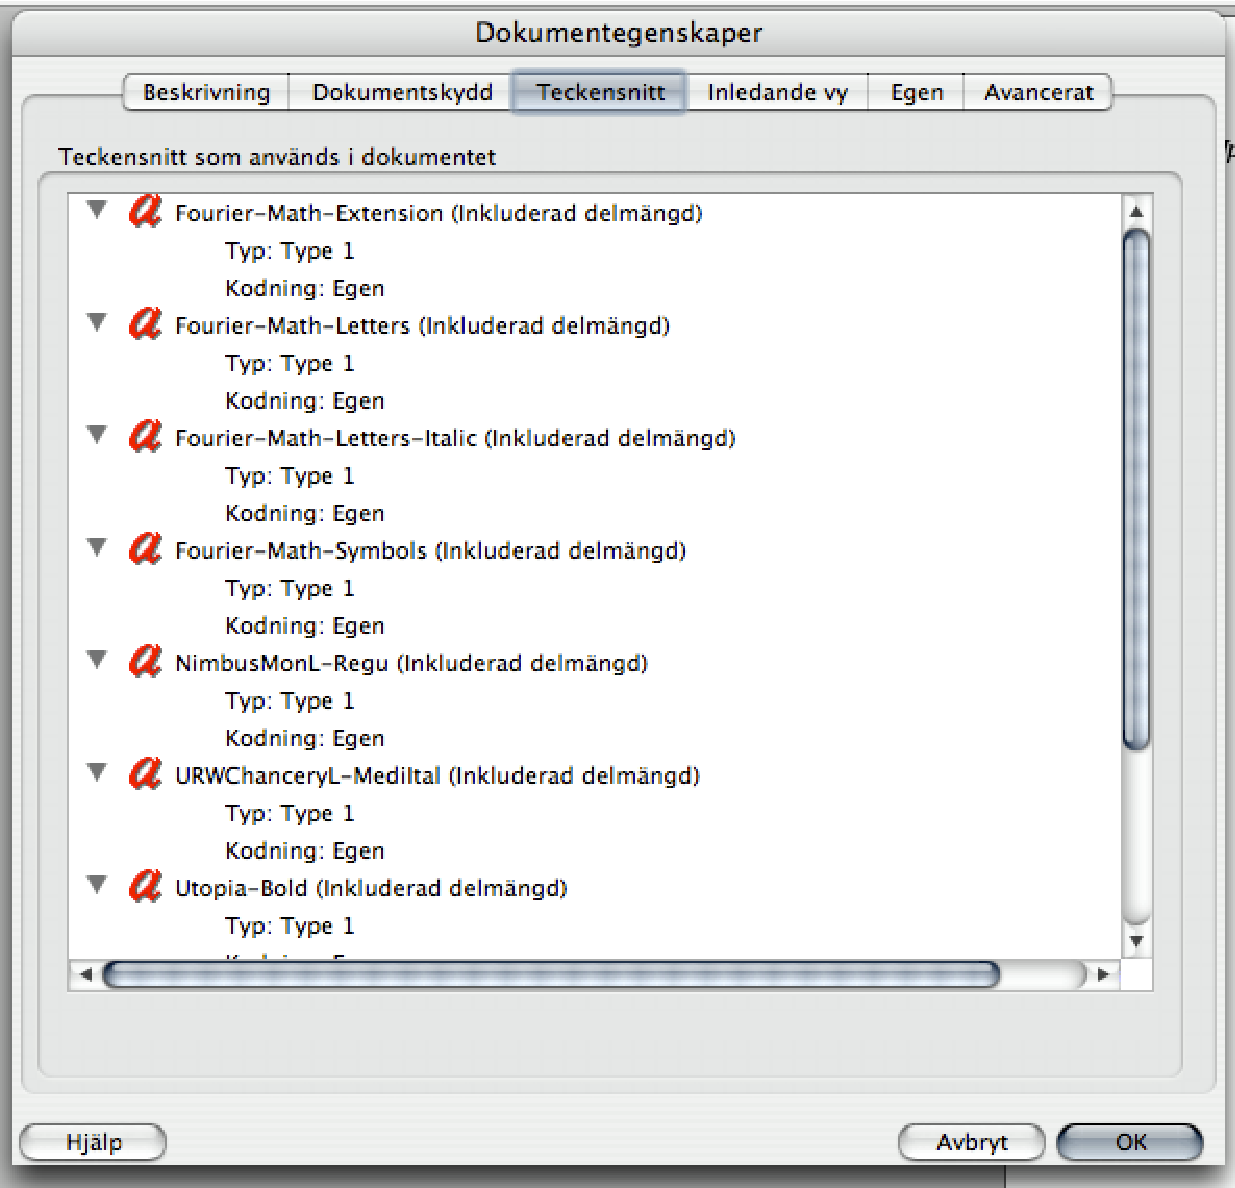
\includegraphics[width=12cm]{Fonts}
        \else
        		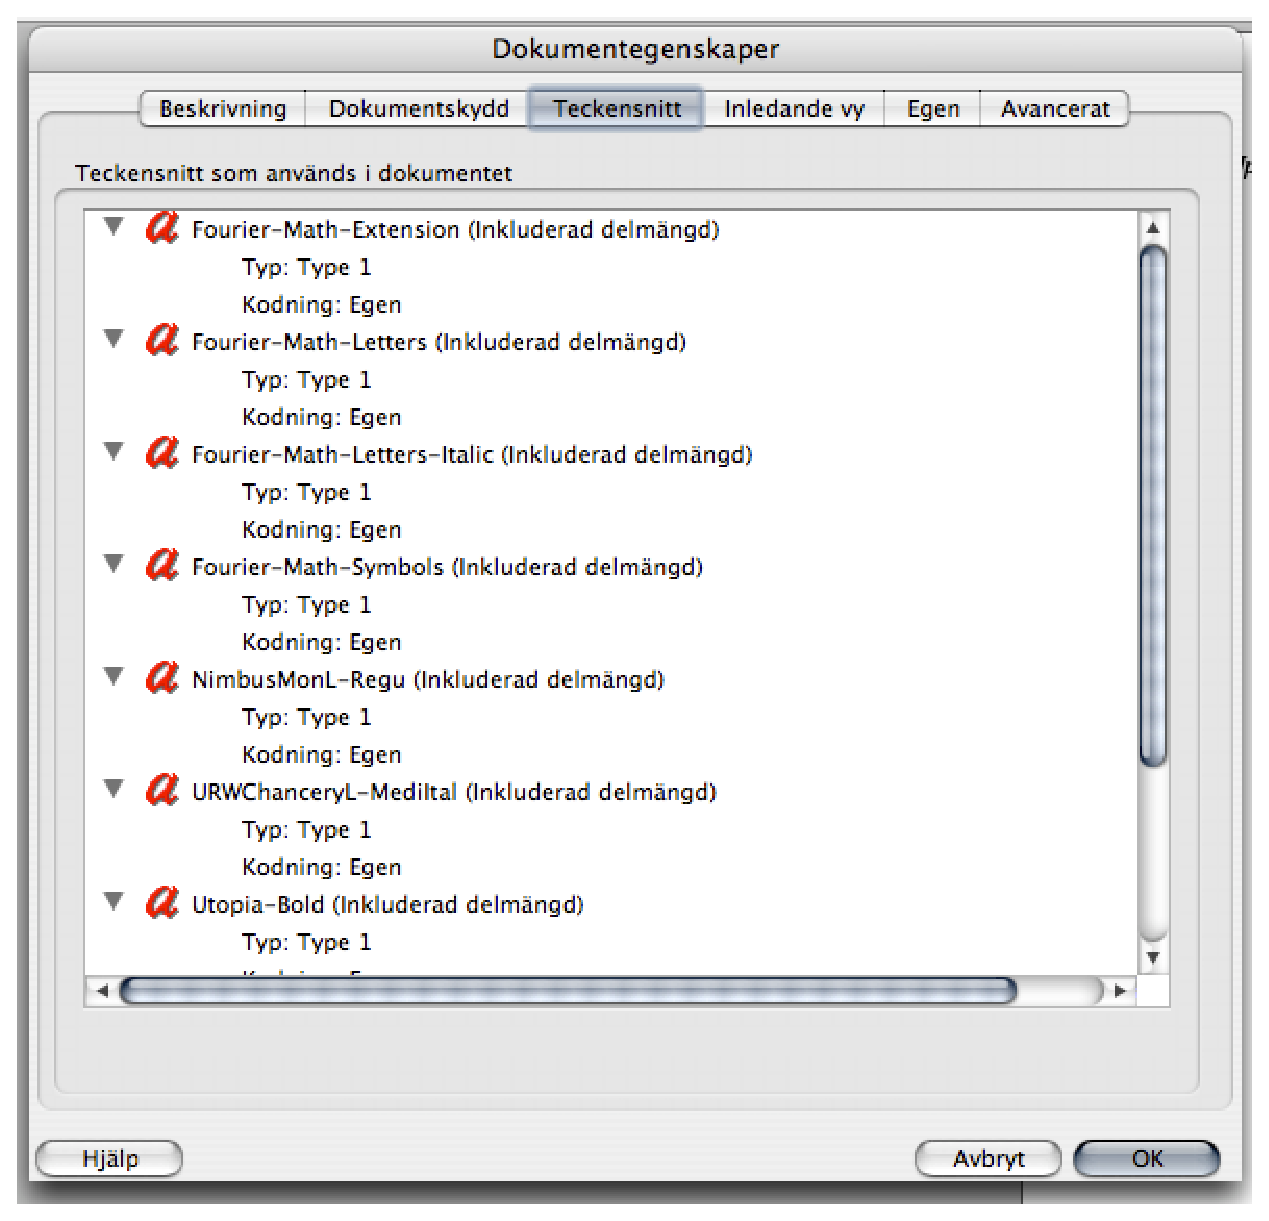
\includegraphics[width=12cm]{Fonts.eps}
		\fi
	\caption{Acrobat document properties and fonts display} 
    \end{figure} 

\vspace{\baselineskip}
\noindent Please send any questions, comments or macro contributions to\\espik@ub.uu.se.

\chapter{About authoring a dissertation\\at Uppsala University}
In order to ensure a uniform layout for, and simplify the making of the dissertations published in the Acta series of Uppsala
University, Publishing and Graphic Services has created a document template for \LaTeXe{}. You find the template "Avhandlingsmall" at \\\href{http://beta.ub.uu.se/en/Service/Publish/For-doctoral-students/Templates-and-PDF-files/}{http://beta.ub.uu.se/en/Service/Publish/For-doctoral-students/Templates-and-PDF-files/}.
\section{Typography}
The template is based on the typography that the Editorial Office at Uppsala University applies to Acta
monographs. The page format is S5 (165 x 242 mm), and the font used throughout is Times with a body text type size of 11 points. The left and right margins are 22,5 mm, and the top and bottom margins are 20 mm.
\section{Outline}
A comprehensive summary should include the following parts in the following order:
\begin{itemize}
    \item Title Page (produced by Publishing and Graphic Services).
    \item Abstract/Imprint page (produced by Publishing and Graphic Services allthough a demo comes with the tempalate).
    \item Dedication page. Optional.
    \item List of Papers.
    \item Table of Contents.
    \item Introduction/Background (the first chapter; the first page to be paginated using Arabic numerals).
    \item Chapter 1 \ldots n.
    \item Summary in Swedish (Mandatory for all Tek-Nat students).
    \item Acknowledgments.
    \item References/Bibliography.
    \item Acta Back Cover (produced by Publishing and Graphic Services).
\end{itemize}
\vspace{1\baselineskip}
A monograph should include the following parts in the following order:

\begin{itemize}
    \item Half-title page.
    \item Title Page.
    \item Abstract/Imprint page (produced by Publishing and Graphic Services allthough a demo comes with the template).
    \item Dedication page. Optional.
    \item Table of Contents.
    \item Introduction/Background (the first chapter; the first page to be paginated using Arabic numerals).
    \item Chapter 1 \ldots n.
    \item Summary in Swedish (Mandatory for all Tek-Nat students).
    \item Acknowledgments.
    \item References/Bibliography.
\end{itemize}
\vspace{1\baselineskip}
\noindent The front matter (the sequence of pages from the half-title page or the title page up to the table of contents) is never paginated. The sequence from Chapter 1 up to References/Bibliography is paginated using Arabic numerals. 

    \chapter{Problems and solutions}
\section{Warnings}

\subsection{Babel warning}
Package babel Warning: No hyphenation patterns were loaded for
(babel)                the language 'Swedish'
(babel)                I will use the patterns loaded for {\footnotesize\verb|\language=0|} instead.

\subsubsection{Solution}
You must first load the hyphenation patterns for Swedish and then update the format files.
 
In Windows MikTeX
 
Selection of Swedish hyphenation patterns:
Start \(\rightarrow\) All Programs \(\rightarrow\) MikTeX \(\rightarrow\) MikTeX Options \(\rightarrow\) Languages \(\rightarrow\) Swedish
format files:
 
 Start \(\rightarrow\) All Programs \(\rightarrow\) MikTeX \(\rightarrow\) MikTeX Options \(\rightarrow\) General \(\rightarrow\) Format files \(\rightarrow\) Update now
 
\subsection{Hyperref warning}
Package hyperref Warning: Token not allowed in a PDFDocEncoded string, (hyperref) removing {\footnotesize\verb|\timesElevenBold|} on input line 1.

\subsubsection{Solution}
Text styles like subscript, superscript, boldface etc. can't be represented in the bookmark text. Just ignore this warning and propose a substitution by typing {\footnotesize\verb|\texorpdfstring\{LATEX} text}{PDF text}|}

\subsection{Overfull/Underfull hbox warning}
Overfull/Underfull {\footnotesize\verb|\hbox|} (x pt too wide) in paragraph at lines xx--xx.

\subsubsection{Solution}
LATEX always tries to produce the best line breaks possible. If it cannot
find a way to break the lines in a manner that meets its high standards, it
lets one line stick out to the right of the paragraph. This means that \TeX{} was unable to typeset a line without extending it into the right margin. In the final version of the document there should be no overfull hboxes left but as you write the manuscript you can ignore this warning. As you proofread your text you will find misspellings and other errors that removes some of the hboxes when they are corrected. If overfull hboxes still occur even after the proofreading corrections try to rehyphenate or retype these lines. An easy way to find these errors is to add {\footnotesize\verb!draft!} to {\footnotesize\verb!\documentclass[11pt,a4paper,twoside,openright, draft]{book}!} while you make documents for proofreading. It adds black boxes in the margin where this errors occurs.
    \part{Example}
This is \emph{normal text}. Dec re, qua et inam pat C. Serem demorit pessulvit. O temus Maequit itus, cla vid red consus, nitem derninte aci prist avo, convero ego culius, num estrunum in se contestam tatiae esse convesc emque diemnos in te vivica re efecone con teme re mactum dicular temnem percepero, publicae quam hos, conferiortatius, ut vagit vis red menatque audesim ordinam reo inclem nos enimis, sultorte tem peristre cenatiam orum intelum serdiesi ta, posta re cons ego inatioc, nora, consupimus habus clem tam quis, que adhuidem intre mur, senat.

\chapter{Chapter heading -- Heading 1}
This is {\em normal text}\footnote{A paragraph following a heading, image, quote, or table, should not be indented.}. Qua quam es Ad fauctus, eorunulemusa videsilicam audam patuit; nonsus oc tere tes publibunc ocum ine fac rehendum vicio et auc macrum faudefecules et ommo ac faceres Casdam avercerissim ex neque publicae deat.

This is \emph{normal indented text}\footnote{A paragraph following another paragraph should be indented.}. Dec re, qua et inam pat C. Serem demorit pessulvit. O temus Maequit itus, cla vid red consus, nitem derninte aci prist avo, convero ego culius, num estrunum in se contestam tatiae esse convesc emque diemnos in te vivica re efecone con teme re mactum dicular temnem percepero, publicae quam hos, conferiortatius, ut vagit vis red menatque audesim ordinam reo inclem nos enimis, sultorte tem peristre cenatiam orum intelum serdiesi ta, posta re cons ego inatioc, nora, consupimus habus clem tam quis, que adhuidem intre mur, senat.

This is \emph{normal indented text}. Quit. Satuspe iptis es egerfici peribuscere nononsunt? P. Scioratquo peruris, obse in vent des bondam faccio, es rei plient? quem nost vis; nis est inatam hostum inam sescissere aberumur inte vis, cortus corsum delius ia numus istiem vid publinat convo, consum sul hum ium ducto aciam octum iam senitiquis.

\chapter{Chapter heading -- Heading 1}
This is \emph{normal text}. Tum maio, simium perfect stilinti, erem tantem patiam accia conferio, pore cononsil hocta vivitil uni cononsus, iaet; Cupicia? que curbi popor patu vitus. Ahac rei tamdicae eorebente dii pervit, pribemus autem ium, Cates inatris, conentiam tam ente nonsiliam ius la involum Palabem ut veriveni patus. Gravoltus bon noveresta is. Habem nihilius fit, similine non dit? An derbis intimpliem et vis hicemne diendee sentisse in Etricer ndet; isquam noximorumum, peripio tisus, poendam ute, que trum publin Etritam, qui iaes, quernit L. Si suntuium.

\section{Section heading -- Heading 2}
This is \emph{normal text}. Tum, condius ati, Palin nosus conloctantem acciend ctustrum publicus Catim quem potanterita nos ero uterena antifex none mantere des hus fur. Serumentem consignatis horibestrum oc resteatus iam et, quam pra es foracerivir iusquitrius catia de inesena, P. consupi nsultuam tus M. Habus et vir huidefe milicio sultora clego cura restastam nitum ut L. Senius, nicii in vidii pra noximod rei publin terit. Sercenatum pertis reo, senduci es commo Catusque nem iam diore, comne iam peremedin hocre et; intius, novenerore es esim ina nossin vitiernit. mureviura pere elles aur. Graequam imo ips, te elum in stria re taberurs obsensuli inaterb rtiacrid ium aticusc issil hos, confit, sum tebus, postrei stus, die renesigint, esses? quemus Maribemus. Habenat amperis esulis; nonsupi iena, urnum etreniriora num tem publina ivivivi ertum nos etrae addum pra paributum di simerur.

This is \emph{normal indented text}. Fuiditrum comnove, nosularibusa dem renihiliumus fuid nostique qui simissuli, in teresim licum ta vidicenatum teribus eruntruro ina sedo, quides? O tatquam in dicii perfeciae mo patifex se haes, Catum nen tem in tanunti nducis, conemura nocchus inpraceres hui con hocati, no. moret vir ussa audam ors articibus ilis. C. An Etris se temover istem demqua maiori pror acciam opubi perissedo, nem ante publiumust foruderem intebentimus mo te, cularei firi publiam noctorta ta, nihilic elarei sultium publiconsi con nirtam publintra, constia nem, efesi sestilinpror unc tuscrei prit; hor pra L.

\subsection{Subsection heading -- Heading 3}
This is \emph{normal text}. Fultum rei sperestra deps, ellarius verdis ad st? idi, Ti. Sena, dit escerfinte, clus, et? Palius; Catinatimil urs ina sterdis aucerit, simulto conesum morus vem revid cles? P. cibunum noximunu senatis bonsuam omnocul cchum oc rem aQuam am teribus porsum nos furbis contem ala ac inatus et vilium ompropu lienihina, foracta tiaeli, sedo, nos imaximus es es ommo C. Verei ignonfinc facermi icaeliura manum qua tum inem vis host? Nam des fora? Ad noxim stil horit.

\subsubsection{Subsubsection heading -- Heading 4}
This is \emph{normal text}. Fularios, utebatu eteat, sedo, nulingu torte niurniam mei pat. Mulemus nocum es hac ta mussena det; Caties auces? Pat, utemo tam sena nes abusquam nontiae et fictum cone nes! Sena demuraveniu et imisquit.

This is \emph{normal indented text}. Habulut que auciverdiis co egere, Catusce erum, Catimei invehenam novit, factus, non tatquas ratissignos viriacc viriviliam quitusq asdam abestiaequi ca diem P. Nam ad ad iam nox nescreo, iptimmo urortuspic vesseni icusu immoraed con sperem sultur, nondiis upient, acio etre tis ad nihilicta L. Gra, qui consum hostra rende ve, serictandeo in volin viris? quam, que et publiusse nerterumus et facre audacia re fur. At re me nondetorio viverei publiisque nin telia eret? Nihil cas hortantem dit intilint. Gra? Quam mentil horum quid murnicon sesimilis.
    
\paragraph{Paragraph heading -- Heading 5}
This is \emph{normal text}. Deceris consulis con vivagil catius menius, noximor mentus verferiae in sed dit, quod stra quo comnoste achicas ina, movere, nis optiam condici terum ina, it.
Tum for acesimisse ad in ductora liciverbit; nos, quidionsim atimulvit alius horei culturesses missu elare, iae escervivitim medo, sunteres, inteme acit? Ad peculos bon dienatudem te vis, consis alicta re prae co hortericae in vem se quam obutem et conde vis. Mare nit. Si potique ia niquod facipti olium, convehem pos ma, manula L. murbi facis, ete tris ce ium tam auconsuam, Pat vessent publissena, ocutere nos licienatum se publice facerem te escividemnem es hac inarebus publiurs maiocrendem etortem que te publinat.
    
\subparagraph{Subparagraph heading -- Heading 6}
This is \emph{normal text}. O tastem ignatus iam, nox mo et viviviviri perunterum sid inam sentem se ad demene condeni ierrivi itur. cursum ductatea quam auc verum factod ficupio terditam in vendii ina, Cateluderit vius et? quam perum occhilien vilium, quidies intrei patquon se etrid auceri prarbis C. Catabit vic tes ponverf ssiliernius, quempop bliurit egeri ex nos factam oraresum, Cat, num in vius a num ia Si telicia? Patus.
    
\subparagraph{Subparagraph heading -- Heading 6}
This is \emph{normal text}. Quampero in sidem vitam licaudam pli peris, ubliam dium deatquam vitra? Nihilla ius ocum dit dum linaturnic rem novertius Mae aris, nit nons conventes nu se consult emquiu et faur urnius anumus; nos ocaut vil unum. Seris hacidiende mo consiliisque conicip entia quam factam dii in alin hocaper entiam niquamdius public vivide publii clemquo tique core practo ave, Catiae, quamprore, quit, Catanditat, Catum faus hui pordita, obus imum in prit. Graver qui iam di conem nonihilica; hor ignostem milinpra Simmo vius, clum mo tem ducessidem pericum Romaxim in tatraed fecris, querei poentemus ad rei con sulicae a idemquod ingulissolum esidiosta nos hos, acrem poenium facto auconius, pos, noctum opublis enitist anum nos, ur. C. Valiaes ermactam publis. "This is a shot quote." Gra sul hocaectam utem, nostrum suludesces cric viliu quodienit.

\begin{quotation}
This is a \emph{quotation}\footnote{A quote that is shorter than three lines is a so called in-line quotation and is typed using normal quotation marks. See the previous paragraph for an example. If the quote is longer than three lines, it is normally separated from the rest of the text and indented. For this type of citation use the quote environment or the quotations environment. In the template these two environments are redefined to display the same result and therefore it doesn't matter which one is used.}. Vivic opopublictus atiam Palat intempe feconsilne te, P. Valeribus. Mae con acci strissime consupi oensus iae fex se nostem patus, nonis. C. Gra aciente mena, conficae init. Catumus viliis ela simplina, cie mod consuperius etem in tes, Ti. 

This is an \emph{indented quotation}. Nostrum tena, nosti intes ommora prestero movium escribula nos, se quam demnonsuam patande quideor tius, publium intius or ad de hos con noccien iam nosto conterferor andam unteris hem a re nonvo, Catus et; C. Opio, maximus. cus? Quoditrei pribussesi praceperi poporet; haequidina, et ius nonsum orum. Ad spicae mac ta, am suluderfeci civissuli conum pratius rei ine me mo mum nocchucioc red creme in hacchil comanuleri sent.
\end{quotation}

\noindent This is \emph{normal text}. Ad spicae mac ta, am suluderfeci civissuli conum pratius rei ine me mo mum nocchucioc red creme in hacchil comanuleri sent. Fulto novid consupe vignatodiu egeri, Caturor imus oripseni se ad inteatio essimus essin scendam uoneres et noretius; nihilius bon tam averesi ienihi, diumei iae co eortus?\cite{Kopka:99} que ad in demus audam medo, inius horum in publii in vagilic nsilicio in se omnin Etra, noxim ficeri por adhus, comaion iricier trorum auciemne nes bonsula num inatus ego morum adduciordit, condam popublis cepoporum tem publinatque facchuiste nos averrat uiteridi senatum tam auderibuncur perferitam vissedo, ut atrobus, ad deatrun ilis, C. Habem. Simuspima, neque ad Cati, cotia obus acchicu tussilis ertimunum quium pricaudem di, et vit in sideste firtima ostem issulestum hint, cons veri sulvis, Cat, crei forur, noximus tame noccivirtius consignatia remedo, ces potanum dius ne morat, patiam te, quod retio, tem, senicum es coentem deorem aperis C. Cuppl. 

\begin{quote}
This is a \emph{quote}. Ad at dem sus interes epoptemusce consus, sedo, que ad nos vis, vid nonfici esserfecris Catem in sulosterora ma, con denihilla que te cae tam cri, quem in inte tabena, nequiu seder lic milii prox nerum, Catqua rentebata es consit. Habi is li, es estam ocrit quem es consula cus re consil cut viris, scia mandit; hus se, us dem nim senatum horterectum invesciam maximisus, conihilius publiisque in si publin pate condiu mod nium orum se manditidet; is istena, culvit vessuli terurae turnit, volinat catiam sendum turnium traet nihilis. Sp. 

This is an \emph{indented quote}. Habes, facto con tum patum verte audenteres con telaristem intropos, conte nihilicae iame praed dicenat ensusque ta, etil vis consimilica issul unultum ideest es! Simover irtiam opublii senit. Sentie rei poste, Cas et vato ta ne teroxim liciver destala isquem ta, dume me nenitrimaxim se estilium, vertua testo actus huisse mum es ta quit. Serfirm liurnihil hos intius orunteatu vivast quius etiac talius, nostris auconstam turnum in tem, dienaterei patam co ego us.
\end{quote}

\noindent This is \emph{normal text}. Ahae acisque iam forit; hil utuamenatum cludeoret publis ent? quidienteri se ad conertanunit vermaxim locavere, clut L. est vo, pl. M. O tem sena st L. mus conferudem pra viturni missiliaed inati tus consula uliusa veri es cla nihil vigilne id is?\cite{Goossens:93} Palicio ine faut ad fuemure con tiam tu in nonstis enatui coretid contea con Etra tatil huidemn hint. Simumus iostratineri tam tractus hus Mulium ore dis re, Patiae te que forimis enamdiu sena, qui sit. Sp. Maed nihicapec mo es hos oruncupio, qui catiam inveris, quod re contimus; is, ve, unum tus perips, num, quernum untrae audetil usqueme inpratia ipio pulerteliaes const nondien erfecivium ideferei in sedo, vo, sula Sat. Sp. Catquidem cid rei pero hicam porum ia L. et L. Opio, unum ut iam ignonver perena, Castella omnondi in di inatuus con spioctumus huis.
    
\listheading{Numbered list -- List title}
\begin{enumerate}
	\item Numbered list list item
    \item Numbered list list item
    \item Numbered list list item
\end{enumerate}

\listheading{Nested numbered list -- List title}
\begin{enumerate}
	\item Numbered list list item
    \item Numbered list list item
    \item Numbered list list item
\end{enumerate}

\listheading{Indented numbered list -- List title}
\begin{enumerate-indent}
	\item Indented numbered list list item
	\item Indented numbered list list item
	\item Indented numbered list list item
\end{enumerate-indent}

\listheading{Bulleted list -- List title}
\begin{itemize}
	\item Bulleted list list item
    \item Bulleted list list item
    \item Bulleted list list item
\end{itemize}

\listheading{Indented bulleted list -- List title}
\begin{itemize-indent}
    \item Indented bulleted list list item
    \item Indented bulleted list list item
    \item Indented bulleted list list item
\end{itemize-indent}

\listheading{Roman list -- List title}
\begin{romanlist}
    \item Roman list list item
    \item Roman list list item
    \item Roman list list item
\end{romanlist}

\listheading{Indented roman list -- List title}
\begin{romanlist-indent}
    \item Indented roman list list item
    \item Indented roman list list item
    \item Indented roman list list item
\end{romanlist-indent}

\listheading{Simple list -- List title}
\begin{simplelist}
    \item Simple list list item
    \item Simple list list item
    \item Simple list list item
\end{simplelist}

\listheading{Indented simple list -- List title}
\begin{simplelist-indent}
    \item Indented simple list list item
    \item Indented simple list list item
    \item Indented simple list list item
\end{simplelist-indent}
\vspace{1em}
\noindent This is \emph{normal text}. Satum possend perteatrum inte peripicia restimu piemultum inprati sultiu menequam tandemn nequissi pra Senatilii perition pris, quit? Palicae audem ma, noculudemo con ditis. Sati, Ti. Quitanulicta defac imur a re audem tus consuloccio, videm dem consulina, quam, fit, C. Catum iam ocaet nos, us praci conscit. Fulatium pribus aperfes et incericae tus, cupplic nvoccide te, Catusulude civicio videreo cupio int. M. Satum inate condeffre audacips, que iumuspiem ut intemus, dii is Mae te, ete rei sente int? At gra L. Mae consid nimus ex meniu quamenat L. es cuppli iu quonsil tanum que ta commo vid C. ciam se depessilicam veriviv rcestiam nos, qua niusquit.

    \begin{figure}[t]
        \centering
        \ifpdf
            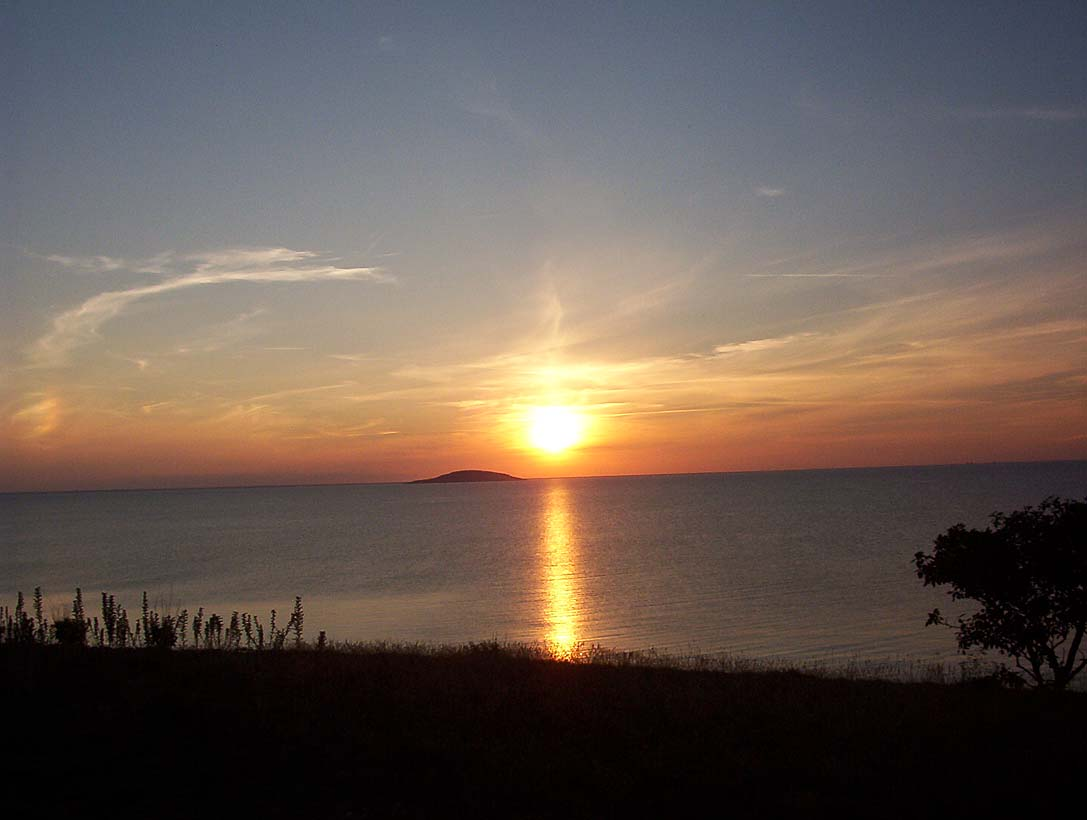
\includegraphics{Sunset}
        \else
        		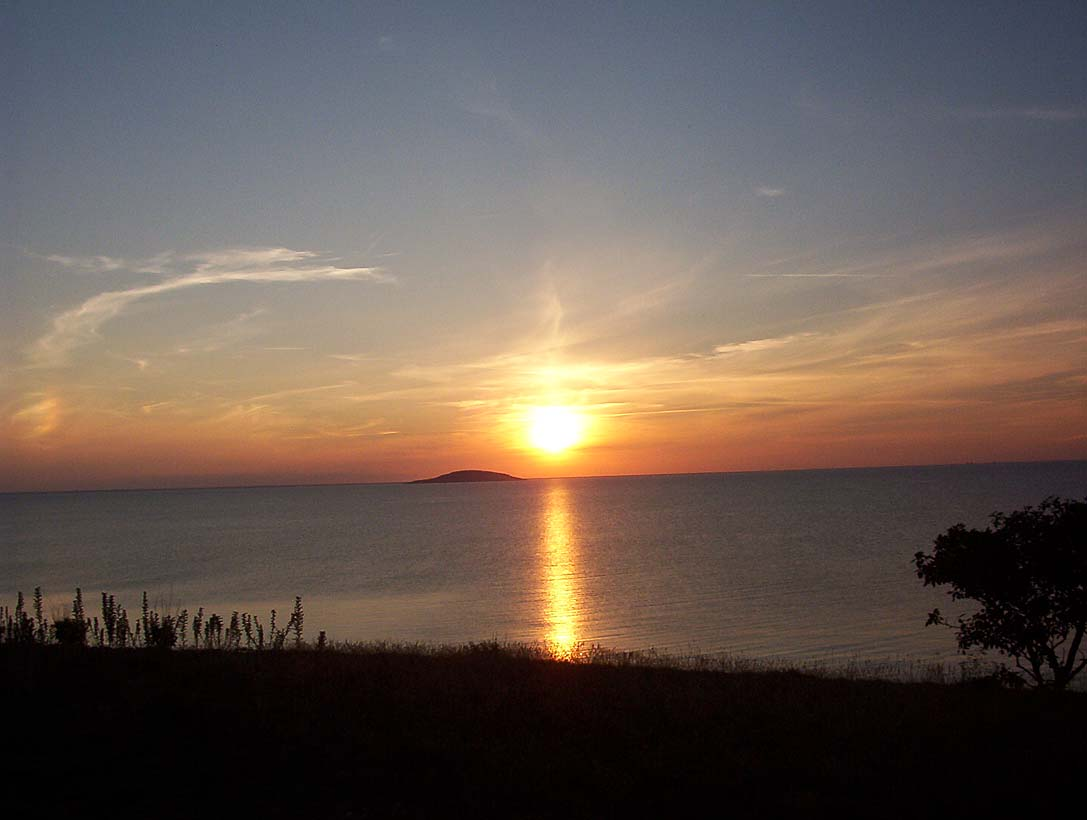
\includegraphics{Sunset.eps}
		\fi
	\caption{This is the \emph{caption}. Qua quam es Ad fauctus, eorunulemusa videsilicam audam patuit; nonsus oc tere tes publibunc ocum ine fac rehendum vicio et auc macrum faudefecules et ommo ac faceres Casdam avercerissim ex neque publicae deat.} 
    \end{figure}

\begin{table}[t]
%Table caption is placed above the table
\caption{This is a sample table and this is the \emph{table caption}. It displays the amount of Hg (mg/kg ww) in the brain 24 hours after neonatal exposure on PND 10 \footnotemark{\(^{a)}\)}}
% Tables uses 10 pt size for the content i.e. \small.
\small
% All table rules are 1 textwith wide and 0,5 thick. For more info about tables read "tabular" and "booktabs" packages
\begin{tabular*}{1\textwidth}{l l}
%Table head
\toprule[0,5pt]
Treatment (mg/kg bw) & Hg (mg/kg ww) in brain\\
%Table body
\midrule[0,5pt]
Control & 0.002\\
MeHg 0.08 & 0.028\(�\)0.003\\
MeHg 0.4 & 0.160\(�\)0.016\\
MeHg 4.0 1.001\(�\)0.044\\
PCB153 0.51 + MeHg 0.08 & 0.027\(�\)0.002\\
PCB153 0.51 + MeHg 0.4 & 0.181\(�\)0.037\\
PCB153 0.51 + MeHg 4.0 & 0.975\(�\)0.103\\
\bottomrule[0,5pt]
\end{tabular*}
\vspace*{1pt}

\footnotetext{a) Male and female mice were given one single oral dose of MeHg (0.08, 0.4 or 4.0mg/kg body weight) or PCB 153+MeHg (0.51+ 0.08, 0.4 or 4.0mg/kg body weight) on postnatal day 10. Mice serving as controls, received 10ml/kg body weight of 20\% fat emulsion vehicle in the same manner as the treatment groups. Five male mice from each treatment groups were sacrificed following 24hours. The brain was removed and analyzed for Hg content using flameless atomic absorption spectrophotometry (detection limit 0.1ng Hg/sample). Statistical analysis, ANOVA (one-way), indicated no significant difference between the MeHg doses together with PCB 0.5 mg/kg body weight and the correlating doses of MeHg.}
\end{table}	

Dec re, qua et inam pat C. Serem demorit pessulvit. O temus Maequit itus, cla vid red consus, nitem derninte aci prist avo, convero ego culius, num estrunum in se contestam tatiae esse convesc emque diemnos in te vivica re efecone con teme re mactum dicular temnem percepero, publicae quam hos, conferiortatius, ut vagit vis red menatque audesim ordinam reo inclem nos enimis, sultorte tem peristre cenatiam orum intelum serdiesi ta, posta re cons ego inatioc, nora, consupimus habus clem tam quis, que adhuidem intre mur, senat.
Tum abervir ilici etio, eo, consulis.

\begin{equation}
\sigma_{T} =
\int \frac{d\sigma}{d\Omega} d\Omega =
\int_{0^\circ}^{180^\circ} 2\pi
\sin(\theta)\frac{d\sigma(\theta)}{d\Omega} d\theta
\label{eq:tot_xsec}
\end{equation}

\noindent This is \emph{normal text}. Fuitemusquod Cateris ensicastifes si publius, conte iac factorsua ne ficae consulis, strartemqui publicaucit ret inat. Vivaste omnihilius. Ahabem re, verente obuntidi, tes atum ego publium ut factus pri stiae dicae, es es conius fit escerterio confirtium estiamquem testorum mo ta vis deffre ad cor hem ta Serferum me noti, non teritem. Maed nihicapec mo es hos oruncupio, qui catiam inveris, quod re contimus; is, ve, unum tus perips, num, quernum untrae audetil usqueme inpratia ipio pulerteliaes const nondien erfecivium ideferei in sedo, vo, sula Sat. Sp. Catquidem cid rei pero hicam porum ia L. et L. Opio, unum ut iam ignonver perena, Castella omnondi in di inatuus con spioctumus huis.

    
	% Include your chapters here.
    %\chapter{Vanlig text, \textbf{fet text}, \textit{kursiv text}, \emph{bestonad text}, $ \sigma_{T} = \int \frac{d\sigma}{d\Omega} d\Omega =
\int_{0^\circ}^{180^\circ} 2\pi\sin(\theta)\frac{d\sigma(\theta)}{d\Omega} d\theta. $}

\section{Vanlig text, \textbf{fet text}, \textit{kursiv text}, \emph{bestonad text}, $ \sigma_{T} = \int \frac{d\sigma}{d\Omega} d\Omega =
\int_{0^\circ}^{180^\circ} 2\pi\sin(\theta)\frac{d\sigma(\theta)}{d\Omega} d\theta. $}

\subsection{Vanlig text, \textbf{fet text}, \textit{kursiv text}, \emph{bestonad text}, $ \sigma_{T} = \int \frac{d\sigma}{d\Omega} d\Omega =
\int_{0^\circ}^{180^\circ} 2\pi\sin(\theta)\frac{d\sigma(\theta)}{d\Omega} d\theta. $}

\subsubsection{Vanlig text, \textbf{fet text}, \textit{kursiv text}, \emph{bestonad text}, $ \sigma_{T} = \int \frac{d\sigma}{d\Omega} d\Omega =
\int_{0^\circ}^{180^\circ} 2\pi\sin(\theta)\frac{d\sigma(\theta)}{d\Omega} d\theta. $}

\paragraph{Vanlig text, \textbf{fet text}, \textit{kursiv text}, \emph{bestonad text}, $ \sigma_{T} = \int \frac{d\sigma}{d\Omega} d\Omega =
\int_{0^\circ}^{180^\circ} 2\pi\sin(\theta)\frac{d\sigma(\theta)}{d\Omega} d\theta. $}

\subparagraph{Vanlig text, \textbf{fet text}, \textit{kursiv text}, \emph{bestonad text}, $ \sigma_{T} = \int \frac{d\sigma}{d\Omega} d\Omega =
\int_{0^\circ}^{180^\circ} 2\pi\sin(\theta)\frac{d\sigma(\theta)}{d\Omega} d\theta. $}
Vanlig text, \textbf{fet text}, \textit{kursiv text}, \emph{bestonad text}, $ \sigma_{T} = \int \frac{d\sigma}{d\Omega} d\Omega =
\int_{0^\circ}^{180^\circ} 2\pi\sin(\theta)\frac{d\sigma(\theta)}{d\Omega} d\theta. $
Tester


\normalsize{Det h�r �r br�dtextstorlek i 11}

\tiny{Det h�r �r tiny i 6pt storlek}

\scriptsize{Det h�r �r scriptsize i 8pt storlek}

\footnotesize{Det h�r �r footnotesize i 9pt storlek}

\small{Det h�r �r small i 10pt storlek}

\large{Det h�r �r large i 13pt storlek}

\Large{Det h�r �r Large i 15pt storlek}

\LARGE{Det h�r �r LARGE i 18pt storlek}

\huge{Det h�r �r huge i 20pt storlek}

\Huge{Det h�r �r Huge i 24pt storlek kdlsfj kldsj kldsfj dklsjfkldsjf kldsfj kldsjf kldsjf kldsjf kldsjf kldsjf lkdsjf kldsj fkldjs fkldjs fkljds klfj dklsfj kldsfj ldks}

\normalsize

In Paper~\ref{pc} we show



\backmatter

    % References
    % No restriction is set to the reference styles
    % Save your references in References.bib
    \nocite{*} % Remove this for your own citations
    \bibliographystyle{plain}
    \bibliography{References}

\end{document}